\documentclass{gduptbe}

%% Info.tex —— 项目实习说明书信息配置
% 参照：过程装备与控制工程专业项目实习设计说明书格式规范

% % Capstone课程偶数页页眉
% \capstoneheader{过程装备与控制工程Capstone课程}
%%=============作者信息=============%
\stunum{xxxxxxxxxxx}
\crest{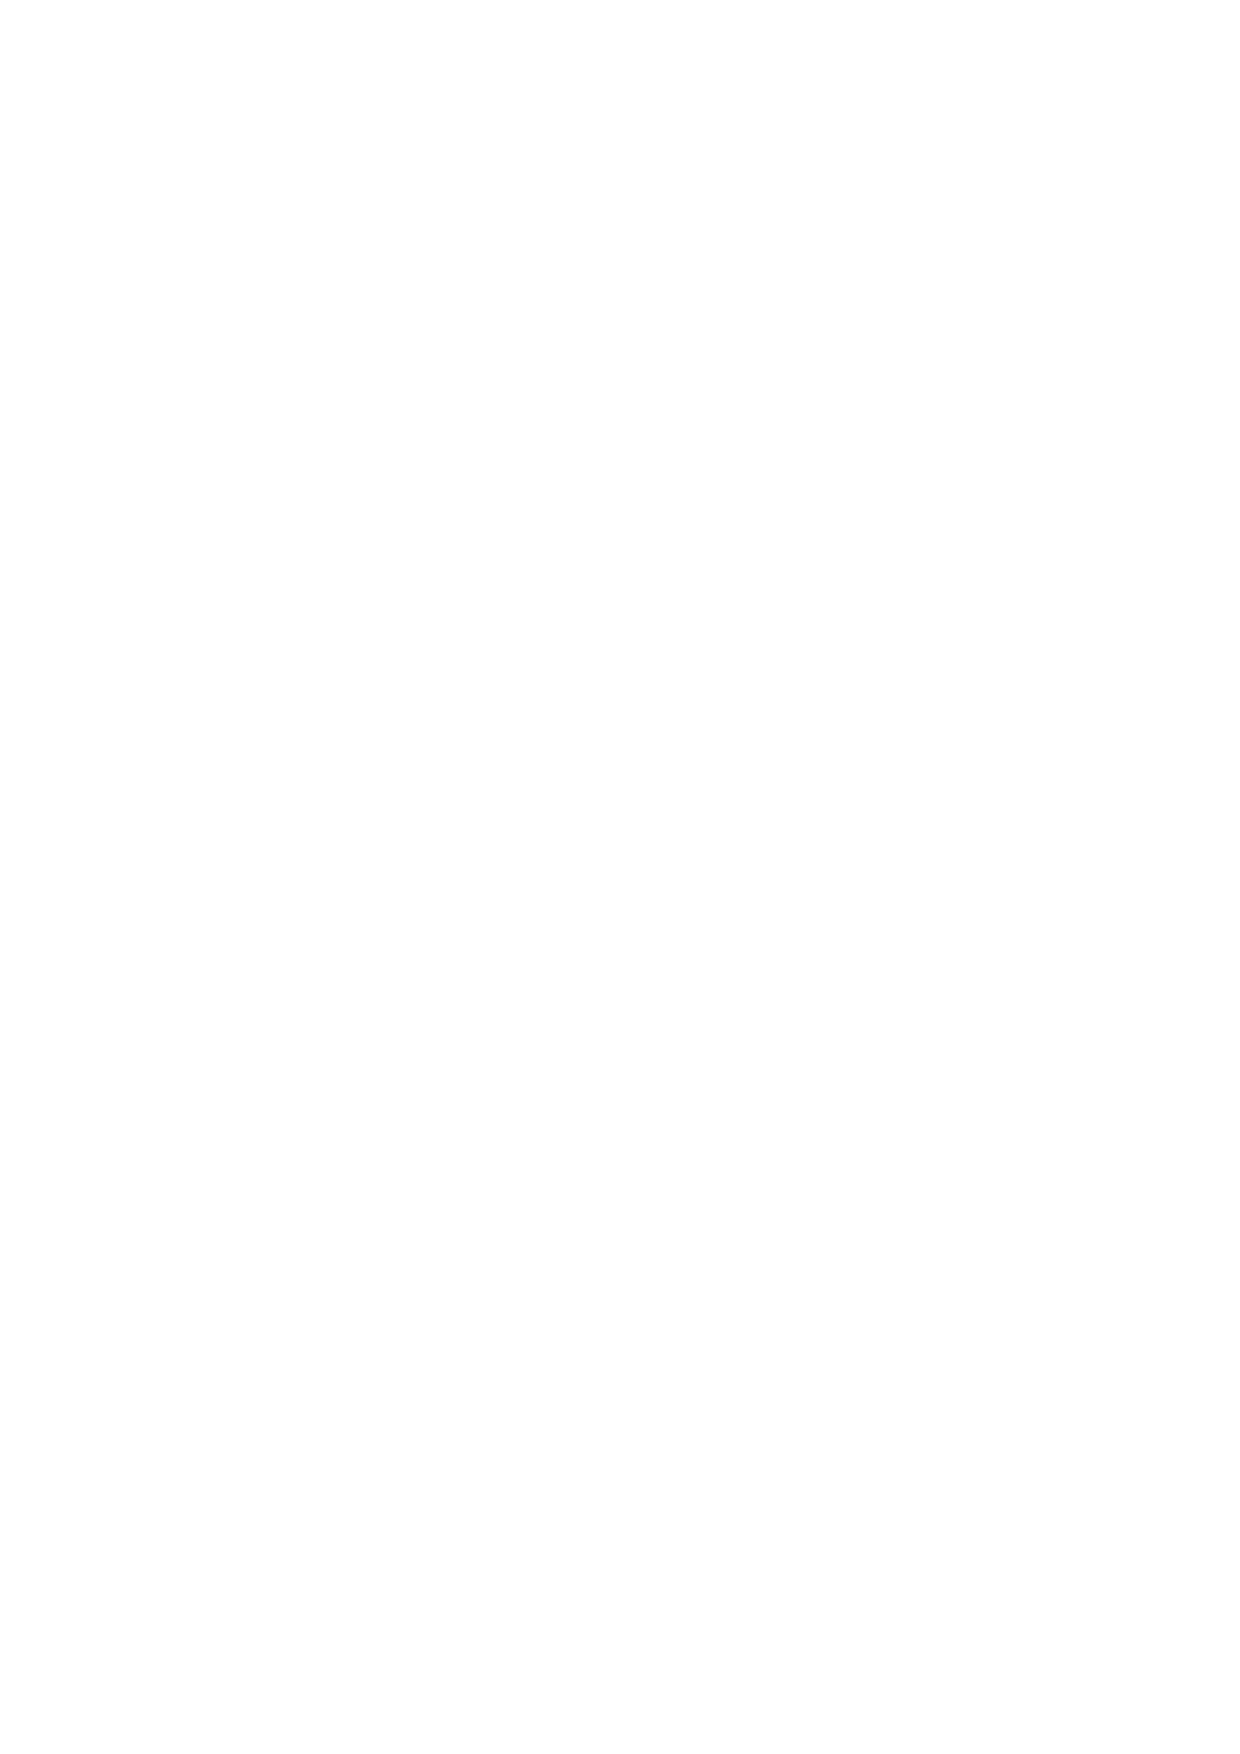
\includegraphics[width=97mm]{imgs/SchoolName}}
\title{\underline{江苏斯尔邦石化冷媒膨胀罐V-1810的机械设计}}
\entitle{\underline{Mechanical Design of Refrigerant Expansion Vessel V-1810} \par \underline{for Jiangsu Sierbang Petrochemical Co., Ltd.}}
%% Subtitle (Optional)
% \subtitle{Using the CUED template}
\author{姓~名}
\advisor{指导教师姓名}
\school{机电}
\dept{过程装备与控制工程}
\stucls{装控23-X}
\designtime{\underline{\makebox[20mm][c]{2026}}年\underline{\makebox[9mm][c]{2}}月\underline{\makebox[9mm][c]{24}}日至\underline{\makebox[20mm][c]{2026}}年\underline{\makebox[9mm][c]{6}}月\underline{\makebox[9mm][c]{20}}日}
%% University 
\university{ 广东石油化工学院 }
% Crest minimum should be 30mm.
%% Submission date
% Default is set as {\monthname[\the\month]\space\the\year}
%\degreedate{September 2014} 

%% Meta information
\subject{冷媒膨胀罐；压力容器；机械设计；强度计算；Q345R} 
% \cnkeywords 和 \enkeywords 在 gduptbe.cls 中未定义，已注释
% 关键词信息已嵌入 parts/abstract.tex 的中英文摘要中
% \cnkeywords{{冷媒膨胀罐} {压力容器} {Q345R} {强度计算} {外压稳定性} {裙式支座} {开孔补强} {GB/T 150}}
% \enkeywords{{Refrigerant expansion vessel} {pressure vessel} {Q345R} {strength calculation} {external pressure stability} {skirt support} {opening reinforcement} {GB/T 150}}


%%=============其他需要的包=============%%

%======= page 页面设置 =============%
\usepackage[top=2.8cm, bottom=2.2cm, outer=2.2cm, inner=2.8cm]{geometry}

% \setCJKmainfont[...]{...}
% ******************************************************************************
% ******************* Fonts (like different typewriter fonts etc.)*************
% Add `customfont' in the document class option to use this section
% \ifsetCustomFont
%   % Set your custom font here and use `customfont' in options. Leave empty to
%   % load computer modern font (default LaTeX font).
%   %\RequirePackage{helvet}

%   % For use with XeLaTeX
%   %  \setmainfont[
%   %    Path              = ./libertine/opentype/,
%   %    Extension         = .otf,
%   %    UprightFont = LinLibertine_R,
%   %    BoldFont = LinLibertine_RZ, % Linux Libertine O Regular Semibold
%   %    ItalicFont = LinLibertine_RI,
%   %    BoldItalicFont = LinLibertine_RZI, % Linux Libertine O Regular Semibold Italic
%   %  ]
%   %  {libertine}
%   %  % load font from system font
%   %  \newfontfamily\libertinesystemfont{Linux Libertine O}
% \fi

% *****************************************************************************
% **************************** Custom Packages ********************************

% ************************* Algorithms and Pseudocode **************************

%\usepackage{algpseudocode}


% ********************Captions and Hyperreferencing / URL **********************

% Captions: This makes captions of figures use a boldfaced small font.
%\RequirePackage[small,bf]{caption}

% \RequirePackage[labelsep=space, tableposition=top]{caption}
% \renewcommand{\figurename}{Fig.} %to support older versions of captions.sty


% *************************** Graphics and figures *****************************

%\usepackage{rotating}
%\usepackage{wrapfig}

% Uncomment the following two lines to force Latex to place the figure.
% Use [H] when including graphics. Note 'H' instead of 'h'
%\usepackage{float}
%\restylefloat{figure}

% Subcaption package is also available in the sty folder you can use that by
% uncommenting the following line
% This is for people stuck with older versions of texlive
%\usepackage{sty/caption/subcaption}
\usepackage{subcaption}

% ********************************** Tables ************************************
\usepackage{booktabs} % For professional looking tables
\usepackage{multirow}

%\usepackage{multicol}
%长表格
\usepackage{longtable}
\usepackage{threeparttable}
%\usepackage{tabularx}


% *********************************** SI Units *********************************
\usepackage{siunitx} % use this package module for SI units


% ******************************* Line Spacing *********************************

% Choose linespacing as appropriate. Default is one-half line spacing as per the
% University guidelines

% \doublespacing
% \onehalfspacing
% \singlespacing


% ************************ Formatting / Footnote *******************************

% Don't break enumeration (etc.) across pages in an ugly manner (default 10000)
%\clubpenalty=500
%\widowpenalty=500

%\usepackage[perpage]{footmisc} %Range of footnote options


% *****************************************************************************
% *************************** Bibliography  and References ********************

%\usepackage{cleveref} %Referencing without need to explicitly state fig /table

% Add `custombib' in the document class option to use this section

%  \RequirePackage[square, sort, numbers, authoryear]{natbib} % CustomBib

% If you would like to use biblatex for your reference management, as opposed to the default `natbibpackage` pass the option `custombib` in the document class. Comment out the previous line to make sure you don't load the natbib package. Uncomment the following lines and specify the location of references.bib file

%\RequirePackage[backend=biber, style=numeric-comp, citestyle=numeric, sorting=nty, natbib=true]{biblatex}
%\addbibresource{References/references} %Location of references.bib only for biblatex, Do not omit the .bib extension from the filename.
\usepackage{gbt7714}

% changes the default name `Bibliography` -> `References'% 参考文献标题：三号粗黑体，居中，上下空一行\renewcommand{\bibname}{\centering\zihao{3}\bfseries\heiti 参考文献\vspace{\baselineskip}}
\renewcommand{\contentsname}{\Large 目\Cspace 录}
\renewcommand{\listfigurename}{\Large 插\Cspace 图}
\renewcommand{\listtablename}{\Large 表\Cspace 格}
\renewcommand{\abstractname}{摘\Cspace 要}

% ******************************************************************************
% ************************* User Defined Commands ******************************
% ******************************************************************************

% *********** To change the name of Table of Contents / LOF and LOT ************

%\renewcommand{\contentsname}{My Table of Contents}
%\renewcommand{\listfigurename}{My List of Figures}
%\renewcommand{\listtablename}{My List of Tables}


% ********************** TOC depth and numbering depth *************************

\setcounter{secnumdepth}{2}
\setcounter{tocdepth}{2}


% ******************************* Nomenclature *********************************

% To change the name of the Nomenclature section, uncomment the following line

%\renewcommand{\nomname}{Symbols}


% ********************************* Appendix ***********************************

% The default value of both \appendixtocname and \appendixpagename is `Appendices'. These names can all be changed via:

%\renewcommand{\appendixtocname}{List of appendices}
%\renewcommand{\appendixname}{Appndx}

% *********************** Configure Draft Mode **********************************

% Uncomment to disable figures in `draft'
%\setkeys{Gin}{draft=true}  % set draft to false to enable figures in `draft'

% These options are active only during the draft mode
% Default text is "Draft"
%\SetDraftText{DRAFT}

% Default Watermark location is top. Location (top/bottom)
%\SetDraftWMPosition{bottom}

% Draft Version - default is v1.0
%\SetDraftVersion{v1.1}

% Draft Text grayscale value (should be between 0-black and 1-white)
% Default value is 0.75
%\SetDraftGrayScale{0.8}


% ******************************** Todo Notes **********************************
%% Uncomment the following lines to have todonotes.

%\ifsetDraft
%	\usepackage[colorinlistoftodos]{todonotes}
%	\newcommand{\mynote}[1]{\todo[author=kks32,size=\small,inline,color=green!40]{#1}}
%\else
%	\newcommand{\mynote}[1]{}
%	\newcommand{\listoftodos}{}
%\fi

% Example todo: \mynote{Hey! I have a note}

% *****************************************************************************
% ******************* Better enumeration my MB*************
\usepackage{enumitem}

% 定义所有的图片文件在 figures 子目录下
\graphicspath{{figs/}}

% % 数学命令
% \newcommand\dif{\mathop{}\!\mathrm{d}}  % 微分符号

% hyperref 宏包在最后调用
\usepackage{hyperref}


% 自适应超宽表格
\usepackage{tabularx}



\begin{document}

\maketitle

%%============= 前导页 =============%%
\frontmatter

% 中英文摘要
% !TeX root = ../thesis.tex

% 中英文摘要和关键字
\begin{cnabstract} 
  以循环冷却水系统的压力缓冲需求为背景，完成冷媒膨胀罐的机械设计。设备采用立式圆筒形焊接结构，筒体内径 1800 mm、切线长度 1700 mm、有效容积 5.85 m³；主体材料 Q345R （正火）钢板，上、下标准椭圆形封头，圆筒形焊制裙座支承。设计遵循 GB/T 150—2024 及 TSG 21-2016，设计压力 $0.80$ MPa(g)（含全真空），设计温度 170 ℃。经计算，筒体与封头名义厚度确定为 14 mm；操作工况环向应力 67.7 MPa，安全系数 2.33；全真空许用外压力 0.125 MPa，水压试验应力 86.3 MPa。
 \\
 \\
 \heiti 关键词：\songti 冷媒膨胀罐；压力容器；Q355R 钢；强度计算；外压稳定性；开孔补强；水压试验
\end{cnabstract} 
  
%%======English Abstract=======%%
\begin{enabstract}
  A refrigerant expansion vessel is designed to meet the pressure-buffering requirements of a recirculating cooling water system. The vessel adopts a vertical cylindrical welded structure with an inner diameter of $1800$~mm, a tangent-to-tangent length of $1700$~mm, and an effective volume of $5.85$~m\textsuperscript{3}. It is constructed of normalized Q355R steel plates, with upper and lower standard elliptical heads and a cylindrical welded skirt support. The design complies with GB/T~150—2024 and TSG~21—2016, with a design pressure of $0.80$~MPa(g) (including full vacuum) and a design temperature of $170$~\textdegree{}C. Through calculation, the nominal thickness of the shell and heads is determined to be $14$~mm; the operating hoop stress is $67.7$~MPa with a safety factor of $2.33$; the allowable external pressure under full vacuum is $0.125$~MPa; the hydrostatic test stress is $86.3$~MPa.
  \\
  \\
  \textbf{Keywords:} Refrigerant expansion vessel; pressure vessel; Q345R steel; strength calculation; external pressure stability; opening reinforcement; hydrostatic test
\end{enabstract}


% 目录
\tableofcontents

%%============= 插图索引 =============%%
% 插图索引（本科生可根据需要决定是否启用）
% \listoffigures

%%============= 表格索引 =============%%
% 表格索引（本科生可根据需要决定是否启用）
% \listoftables

%%============= 符号说明 =============%%
% 符号说明（可选）
% % !TeX root = ../thesis.tex

\begin{denotation}[3cm]
  \item[$P$] 设计压力，MPa
  \item[$P_c$] 计算压力，MPa
  \item[$P_T$] 试验压力，MPa
  \item[$T$] 设计温度，℃
  \item[MDMT] 最低设计金属温度 (Minimum Design Metal Temperature)，℃
  \item[$D_{\mathrm{i}}$] 壳体内径，mm
  \item[$D_o$] 壳体外径，mm
  \item[$L$] 筒体长度（不含封头），mm
  \item[$V$] 容积，m³
  \item[$\delta$] 计算厚度，mm
  \item[$\delta_d$] 设计厚度，mm
  \item[$\delta_{\mathrm{n}}$] 名义厚度，mm
  \item[$\delta_e$] 有效厚度，mm
  \item[$C_1$] 钢板厚度负偏差，mm
  \item[$C_2$] 腐蚀裕量，mm
  \item[$h_{\mathrm{i}}$] 封头曲面深度，mm
  \item[$K$] 椭圆封头形状系数
  \item[$\phi$] 焊接接头系数
  \item[$[\sigma]$] 常温许用应力，MPa
  \item[$[\sigma]^t$] 设计温度许用应力，MPa
  \item[$R_{\text{eL}}$] 材料常温屈服强度，MPa
  \item[$R_m$] 材料抗拉强度，MPa
  \item[$E_t$] 设计温度弹性模量，MPa
  \item[$A$] 外压应变系数
  \item[$[P]$] 许用外压力，MPa
  \item[$\rho$] 介质密度，kg/m³
  \item[$q_0$] 基本风压，N/m²
  \item[LDPE] 低密度聚乙烯 (Low Density Polyethylene)
  \item[EVA] 乙烯-醋酸乙烯酯共聚物 (Ethylene-Vinyl Acetate)
  \item[RT] 射线检测 (Radiographic Testing)
  \item[UT] 超声检测 (Ultrasonic Testing)
  \item[PT] 渗透检测 (Penetrant Testing)
  \item[MT] 磁粉检测 (Magnetic Particle Testing)
  \item[WN] 带颈对焊法兰 (Welding Neck Flange)
  \item[RF] 突面密封面 (Raised Face)
  \item[TOS] 支承基础顶面标高 (Top of Support)
\end{denotation}



% 也可以使用 nomencl 宏包，需要在导言区
% \usepackage{nomencl}
% \makenomenclature

% 在这里输出符号说明
% \printnomenclature[3cm]

% 在正文中的任意为都可以标题
% \nomenclature{PI}{聚酰亚胺}
% \nomenclature{MPI}{聚酰亚胺模型化合物，N-苯基邻苯酰亚胺}
% \nomenclature{PBI}{聚苯并咪唑}
% \nomenclature{MPBI}{聚苯并咪唑模型化合物，N-苯基苯并咪唑}
% \nomenclature{PY}{聚吡咙}
% \nomenclature{PMDA-BDA}{均苯四酸二酐与联苯四胺合成的聚吡咙薄膜}
% \nomenclature{MPY}{聚吡咙模型化合物}
% \nomenclature{As-PPT}{聚苯基不对称三嗪}
% \nomenclature{MAsPPT}{聚苯基不对称三嗪单模型化合物，3,5,6-三苯基-1,2,4-三嗪}
% \nomenclature{DMAsPPT}{聚苯基不对称三嗪双模型化合物（水解实验模型化合物）}
% \nomenclature{S-PPT}{聚苯基对称三嗪}
% \nomenclature{MSPPT}{聚苯基对称三嗪模型化合物，2,4,6-三苯基-1,3,5-三嗪}
% \nomenclature{PPQ}{聚苯基喹噁啉}
% \nomenclature{MPPQ}{聚苯基喹噁啉模型化合物，3,4-二苯基苯并二嗪}
% \nomenclature{HMPI}{聚酰亚胺模型化合物的质子化产物}
% \nomenclature{HMPY}{聚吡咙模型化合物的质子化产物}
% \nomenclature{HMPBI}{聚苯并咪唑模型化合物的质子化产物}
% \nomenclature{HMAsPPT}{聚苯基不对称三嗪模型化合物的质子化产物}
% \nomenclature{HMSPPT}{聚苯基对称三嗪模型化合物的质子化产物}
% \nomenclature{HMPPQ}{聚苯基喹噁啉模型化合物的质子化产物}
% \nomenclature{PDT}{热分解温度}
% \nomenclature{HPLC}{高效液相色谱 (High Performance Liquid Chromatography)}
% \nomenclature{HPCE}{高效毛细管电泳色谱 (High Performance Capillary lectrophoresis)}
% \nomenclature{LC-MS}{液相色谱-质谱联用 (Liquid chromatography-Mass Spectrum)}
% \nomenclature{TIC}{总离子浓度 (Total Ion Content)}
% \nomenclature{\textit{ab initio}}{基于第一原理的量子化学计算方法，常称从头算法}
% \nomenclature{DFT}{密度泛函理论 (Density Functional Theory)}
% \nomenclature{$E_a$}{化学反应的活化能 (Activation Energy)}
% \nomenclature{ZPE}{零点振动能 (Zero Vibration Energy)}
% \nomenclature{PES}{势能面 (Potential Energy Surface)}
% \nomenclature{TS}{过渡态 (Transition State)}
% \nomenclature{TST}{过渡态理论 (Transition State Theory)}
% \nomenclature{$\increment G^\neq$}{活化自由能(Activation Free Energy)}
% \nomenclature{$\kappa$}{传输系数 (Transmission Coefficient)}
% \nomenclature{IRC}{内禀反应坐标 (Intrinsic Reaction Coordinates)}
% \nomenclature{$\nu_i$}{虚频 (Imaginary Frequency)}
% \nomenclature{ONIOM}{分层算法 (Our own N-layered Integrated molecular Orbital and molecular Mechanics)}
% \nomenclature{SCF}{自洽场 (Self-Consistent Field)}
% \nomenclature{SCRF}{自洽反应场 (Self-Consistent Reaction Field)}


%%============= 正 文 =============%%
\mainmatter
\raggedbottom
\songti
% !TeX root = ../thesis.tex

\chapter{工程背景与设计条件}

\section{项目来源与工艺背景}

江苏斯尔邦石化有限公司甲醇制烯烃及烯烃下游一体化一期项目配套冷媒膨胀罐（设备位号：22-V-1810），隶属于 $100\ \text{kt/a}$ 釜式法 $+$ $200\ \text{kt/a}$ 管式法 LDPE/EVA 联合装置（18 单元）。LDPE/EVA 高压聚合工艺的循环冷却水系统在启停、负荷调节及事故工况下，冷媒温度波动引起介质体积变化，需设置膨胀罐以吸纳体积增量、平抑压力脉动并维持循环泵吸入条件\cite{guocheng2020}。

装置建于江苏省连云港市徐圩新区石化产业基地。连云港地处暖温带季风气候区，极端最高气温 $38.5$ ℃，极端最低气温 $-12.3$ ℃。设备露天布置，承受风载荷、地震载荷及环境温度交变作用，设计使用年限 15 年。

膨胀罐在工艺系统中的功能定位明确为三项：其一，利用罐体上部氮气覆盖层的可压缩性，缓冲循环水系统因温度变化引起的压力波动；其二，在变工况条件下向系统补充或回收冷媒，维持循环回路总容积恒定；其三，通过自由液面实现气液分离，防止气体夹带进入循环泵造成气蚀。

\section{设计依据与标准体系}

本设备按固定式压力容器进行设计、制造、检验与验收，遵循的标准体系如表 \ref{tab:main-standards} 所示。

\begin{table}[!htb]
  \centering
  \caption{设计遵循的标准体系}
  \label{tab:main-standards}
  \small\renewcommand{\arraystretch}{1.1}
  \setlength{\tabcolsep}{7pt}
  \begin{tabularx}{\textwidth}{@{}c >{\centering\arraybackslash}X >{\centering\arraybackslash}X@{}}
    \toprule
    \textbf{序号} & \textbf{标准编号} & \textbf{标准名称} \\
    \midrule
    1  & GB/T 150.1～150.4—2024 & 压力容器（主设计标准） \\
    2  & TSG 21—2016           & 固定式压力容器安全技术监察规程 \\
    3  & GB/T 713.1—2023       & 承压设备用钢板和钢带 第1部分：碳钢和低合金钢 \\
    4  & GB/T 709—2019         & 热轧钢板和钢带的尺寸、外形、重量及允许偏差 \\
    5  & GB/T 25198—2010       & 压力容器封头 \\
    6  & NB/T 47065.1-5—2018   & 容器支座 \\
    7  & NB/T 47020～47027—2012 & 压力容器法兰、垫片、紧固件 \\
    8  & HG/T 20592～20635—2009 & 钢制管法兰、垫片和紧固件 \\
    9  & NB/T 11025—2022       & 补强圈 \\
    10 & HG/T 21514—2014       & 钢制人孔和手孔的类型与技术条件 \\
    11 & NB/T 47013.1～.14—2015 & 承压设备无损检测 \\
    12 & HG/T 20580—2020       & 钢制化工容器设计基础规范 \\
    13 & HG/T 20585—2020       & 钢制低温压力容器技术规范 \\
    14 & NB/T 47041—2014       & 塔式容器 \\
    15 & HG 20660—2000         & 压力容器中化学介质毒性危害和爆炸危险程度分类 \\
    \bottomrule
  \end{tabularx}
\end{table}

原始工艺数据取自中国石化工程建设有限公司编制的设备机械数据表（文件号：3767-CD-SE-0V1810\_IS1）\cite{sierbang-datasheet}。设计参数中内径、容积、压力、温度、腐蚀裕量等直接采用数据表给定值；结构型式、材料牌号、计算方法按 GB/T 150—2024 系列标准选取和确定。

\section{操作介质与容器类别}

\subsection{操作介质与介质组别}

本设备操作介质为冷却水（冷媒），在装置正常运行时工作温度 $155$ ℃，设计温度 $170$ ℃。按 HG 20660—2000 的毒性危害与爆炸危险程度分类\cite{hg20660-2000}，冷却水属于无毒、不易燃介质，划入第二组介质\cite{tsg21-2016}。

\subsection{容器类别划分}

依据 TSG 21—2016 附件 A 的分类准则\cite{tsg21-2016}，固定式压力容器按介质组别和压力-容积乘积划分为 Ⅰ、Ⅱ、Ⅲ 三类：

\begin{equation}
PV = P \times V = 0.80 \times 5.5 = 4.4\ \text{MPa}\cdot\text{m}^3
\label{eq:pv-product}
\end{equation}

对照 TSG 21—2016 附件 A 第二组介质分类图，$PV = 4.4\ \text{MPa}\cdot\text{m}^3 < 50\ \text{MPa}\cdot\text{m}^3$，归属第 Ⅰ 类压力容器。本设备按 Ⅰ 类容器进行设计监管，A、B 类焊接接头允许按局部射线检测执行\cite{tsg21-2016}（检测比例 $\ge 20\%$ 且 $\ge 250$ mm），对应焊接接头系数 $\phi = 0.85$（详见第 2 章）。

\section{操作工况与设计条件}

\subsection{操作工况}

设备在两种操作工况下运行。正常操作工况：工作压力 $0.60$ MPa(g)，工作温度 $155$ ℃；温水充液工况：工作温度 $100$ ℃，用于装置开工及检修后系统充液排气操作。此外，设备须具备全真空运行能力，以应对蒸汽冷凝造成系统负压的极端工况。

\subsection{设计条件的确定}

设计压力和设计温度在操作工况基础上附加安全裕量确定，依照 GB/T 150.1—2024 第 3.1 节的原则执行\cite{gbt150-2024}。

设计压力 $P = 0.80$ MPa(g) 的确定：除覆盖正常操作压力 $0.60$ MPa(g) 外，附加操作波动裕量 $0.20$ MPa 以保证压力安全阀的设定值与操作压力之间有合理的压差带；同时计入全真空外压条件（FV，$P_{\text{ext}} = -0.1013$ MPa(g)），设备壳体须同时满足内压强度和外压稳定性的双重约束。

设计温度 $T = 170$ ℃ 的确定：正常操作最高工作温度 $155$ ℃，附加工艺波动裕量 $15$ ℃（含换热不确定因素及控制系统响应延迟），取设计温度 $170$ ℃。该温度高于温水充液工况温度 $100$ ℃，故以 $170$ ℃ 作为各承压元件强度计算的统一金属设计温度。全真空工况对应金属温度 $100$ ℃（蒸汽冷凝工况），用于外压稳定性校核时弹性模量的取值。

最低设计金属温度（MDMT）$-15$ ℃ 按项目所在地极端最低气温 $-12.3$ ℃ 附加 $-2.7$ ℃ 裕量确定，用于材料低温韧性评定\cite{hgt20585-2020}。本 MDMT 高于 Q345R 正火态的最低允许使用温度 $-20$ ℃，材料低温韧性合格，无需额外进行冲击试验。

\section{设计参数汇总}

综合设备机械数据表和标准规范要求，本冷媒膨胀罐（22-V-1810）的全部设计参数汇总如表 \ref{tab:design-summary}。

\begin{table}[!htb]
  \centering
  \caption{设计参数汇总}
  \label{tab:design-summary}
  \small\renewcommand{\arraystretch}{1.1}
  \setlength{\tabcolsep}{6pt}
  \begin{tabularx}{\textwidth}{@{}c >{\centering\arraybackslash}X >{\centering\arraybackslash}X@{}}
    \toprule
    \textbf{序号} & \textbf{参数名称} & \textbf{数值与说明} \\
    \midrule
    1  & 设备位号 / 名称             & 22-V-1810 / 冷媒膨胀罐 \\
    2  & 压力容器类别                & 第 Ⅰ 类（TSG 21—2016） \\
    3  & 操作介质 / 介质组别          & 冷却水（冷媒）/ 第二组介质，无毒、不易燃 \\
    4  & 工作压力（正常操作）         & $0.60$ MPa(g) \\
    5  & 设计压力                    & $0.80$ MPa(g)，含全真空要求（FV） \\
    6  & 工作温度                    & $155$ ℃（正常操作）/ $100$ ℃（温水充液） \\
    7  & 设计温度                    & $170$ ℃ \\
    8  & 全真空工况金属温度           & $100$ ℃ \\
    9  & 最低设计金属温度（MDMT）     & $-15$ ℃ @ $0.85$ MPa(g) \\
    10 & 罐体内径 $D_i$              & $1800$ mm \\
    11 & 筒体圆筒段长度 $L$           & $1700$ mm（切线至切线，不含封头直边段） \\
    12 & 有效容积 $V$                 & $5.5$ m³ \\
    13 & 最大介质密度                & $1000$ kg/m³（满液校核工况） \\
    14 & 壳体/封头材料               & Q345R 正火钢板（GB/T 713.1—2023） \\
    15 & 接管材料                    & 20 号钢无缝钢管（GB 6479—2013） \\
    16 & 焊接接头系数 $\phi$          & $0.85$（A、B 类焊缝，局部 RT，检测比例 $\ge 20\%$） \\
    17 & 钢板厚度负偏差 $C_1$         & $0.30$ mm（GB/T 709—2019 B类偏差，固定下偏差$-0.30$ mm） \\
    18 & 腐蚀裕量 $C_2$               & $3.0$ mm（壳体/封头）；$2.0$ mm（裙座） \\
    19 & 设计使用年限                & 15 年 \\
    20 & 基本风压 $q_0$               & $450$ N/m²（连云港，50 年一遇，B 类粗糙度） \\
    21 & 抗震设防烈度 / 基本加速度    & 7 度 / $0.10g$ \\
    22 & 设计地震分组 / 场地类别      & 第一组 / Ⅱ 类 \\
    \bottomrule
  \end{tabularx}
\end{table}

\section{技术特性表}

按 HG/T 20580—2020 和 TSG 21—2016 的要求，编制冷媒膨胀罐技术特性表（表 \ref{tab:tech-spec}），作为设计说明书和竣工图的首页依据。

\begin{table}[!htb]
  \centering
  \caption{冷媒膨胀罐 V-1810 技术特性表}
  \label{tab:tech-spec}
  \small\renewcommand{\arraystretch}{1.15}
  \setlength{\tabcolsep}{6pt}
  \begin{tabularx}{\textwidth}{@{}l >{\raggedright\arraybackslash}X l >{\raggedright\arraybackslash}X@{}}
    \toprule
    \multicolumn{4}{c}{\textbf{技术特性表}} \\
    \midrule
    设备位号         & 22-V-1810            & 设备名称     & 冷媒膨胀罐 \\
    容器类别         & 第 Ⅰ 类              & 设计标准     & GB/T 150.1$\sim$150.4—2024 \\
    设计使用年限     & 15 年                 & 监管规程     & TSG 21—2016 \\
    \midrule
    设计压力（内压） & $0.80$ MPa(g)         & 设计压力（外压） & 全真空（FV，$-0.1013$ MPa(g)） \\
    工作压力         & $0.60$ MPa(g)         & 安全阀整定压力   & $0.85$ MPa(g) \\
    设计温度         & $170$ ℃               & 工作温度         & $155$ ℃（正常）/ $100$ ℃（温水充液） \\
    MDMT             & $-15$ ℃ @ $0.85$ MPa(g) & 全真空金属温度 & $100$ ℃ \\
    \midrule
    操作介质         & 冷却水（冷媒）        & 介质组别     & 第二组（无毒、不易燃） \\
    介质密度         & $1000$ kg/m³          & 腐蚀裕量     & $3.0$ mm（壳体/封头） \\
    有效容积         & $5.5$ m³              & 充装系数     & $\le 0.90$ \\
    \midrule
    罐体内径 $D_i$   & $1800$ mm             & 筒体长度 $L$（T/T） & $1700$ mm \\
    筒体名义厚度 $\delta_n$ & $14$ mm       & 封头名义厚度 $\delta_{nh}$ & $14$ mm \\
    封头型式         & EHA 标准椭圆封头      & 封头标准     & GB/T 25198—2010\cite{gbt25198-2010} \\
    焊接接头系数 $\phi$ & $0.85$             & 无损检测     & 局部 RT $\ge 20\%$，Ⅲ 级合格 \\
    \midrule
    壳体/封头材料    & Q345R 正火钢板        & 材料标准     & GB/T 713.1—2023 \\
    接管材料         & 20 号钢无缝钢管       & 接管标准     & GB 6479—2013 \\
    裙座材料         & Q345R                 & 地脚螺栓     & M30 $\times$ 400，$n=8$ \\
    设备净重         & $\approx 4245$ kg     & 操作总重     & $\approx 7245$ kg \\
    水压试验压力 $P_T$ & $1.02$ MPa          & 试验介质     & 洁净纯水（$Cl^- \le 25$ mg/L） \\
    \midrule
    基本风压 $q_0$   & $450$ N/m²（50 年一遇） & 地面粗糙度 & B 类 \\
    抗震设防烈度     & 7 度（$0.10g$）      & 设计地震分组 & 第一组，Ⅱ 类场地 \\
    设备布置方式     & 露天，立式，裙座支承  & 保温/保冷    & 不保温 \\
    \bottomrule
  \end{tabularx}
\end{table}
   % 工程背景与设计条件
% !TeX root = ../thesis.tex

\chapter{材料选择与设计基础}

强度计算所需的设计基础参数——材料许用应力、焊接接头系数、厚度附加量及计算压力——在本章中逐一确定。参数的取值直接影响强度计算结果的准确性和设计方案的工程可行性。

\section{壳体与封头材料}

\subsection{材料牌号选择}

壳体与封头材料的选择须同时满足三个约束条件：设计温度 $170\,\textdegree$C 下的强度不显著衰减；MDMT $-15\,\textdegree$C 下的低温韧性；与冷却水介质的化学相容性\cite{gbt150-2024}。

Q345R 是 GB/T 713.1—2023 中压力容器专用 Mn-Nb 系低合金高强度结构钢\cite{gbt713-1-2023}，供货状态为正火态。该钢种在设计温度区间内力学性能稳定性好，在 $-20\,\textdegree$C 以上具备良好的低温冲击韧性，焊接性优良（碳当量 $C_{\mathrm{eq}} \le 0.45\%$，冷裂纹敏感性指数 $P_{\mathrm{cm}} \le 0.28\%$），对工业冷却水（pH 6.5～8.5）的耐均匀腐蚀性能满足设计使用年限 15 年的要求\cite{hgt20580-2020}。

综合以上因素，筒体及封头选用 Q345R 正火镇静钢板，板厚 $3 \sim 16$ mm，其主要力学性能指标和化学成分要求分别列于表 \ref{tab:q345r-properties} 和表 \ref{tab:q345r-chemistry}。

\begin{table}[!htb]
  \centering
  \caption{Q345R 钢板主要力学性能（板厚 $3 \sim 16$ mm，正火态）}
  \label{tab:q345r-properties}
  \small\renewcommand{\arraystretch}{1.05}
  \setlength{\tabcolsep}{5pt}
  \begin{tabularx}{\textwidth}{@{}>{\centering\arraybackslash}X >{\centering\arraybackslash}X >{\centering\arraybackslash}X@{}}
    \toprule
    \textbf{性能指标} & \textbf{符号} & \textbf{数值} \\
    \midrule
    屈服强度（室温）         & $R_{\mathrm{eL}}$ & $345$ MPa \\
    抗拉强度                 & $R_m$           & $510 \sim 640$ MPa \\
    断后伸长率               & $A$             & $\ge 21\%$ \\
    $0\,\textdegree$C 冲击吸收能量 & $KV_2$          & $\ge 41$ J \\
    弯曲试验（$180^\circ$，$d=3a$） & — & 合格 \\
    \bottomrule
  \end{tabularx}
\end{table}
   % 材料选择与设计基础
% !TeX root = ../thesis.tex

\chapter{结构设计与强度计算}

\label{chap:struct-design}

本章在第二章确定的设计基础和材料参数之上，完成承压壳体的结构设计与强度验证。结构设计和强度计算本为一体两面——结构构型的选型决定了计算模型的边界条件，而强度准则的计算结果又反过来约束结构方案的可行性。本章将筒体、封头、裙座等主要承压零部件的结构设计与其强度验证一体化呈现，以工程实践中"设计-校核-迭代"的真实逻辑链展开阐述。

\section{筒体设计}

\subsection{筒体结构方案}

冷媒膨胀罐的筒体采用单层卷焊式圆筒形结构，由一张或两张 Q345R 钢板经冷卷或温卷成形后焊接纵缝，再与上、下封头组焊环缝。该方案在 DN1800 直径级别上工艺成熟，制造成本低，焊缝质量控制手段完备\cite{nbt47013-2015}。

筒体基本参数确定如下：内径取工艺数据表给定值 $D_i = 1800$ mm；切线长度（T/T，不含封头直边段）$L = 1700$ mm，使罐体长径比 $L/D_i \approx 0.94$，属于短粗型立式容器，有利于气液分离和自由液面的稳定；名义厚度 $\delta_n = 14$ mm 的确定过程见本节强度计算。

\subsection{内压强度计算}

筒体计算厚度按照 GB/T 150.3—2024 式(5-1)确定。该式基于薄壁圆筒中径公式，假定环向薄膜应力沿壁厚均匀分布，适用于 $D_o/D_i \le 1.5$（本设备 $D_o/D_i = 1828/1800 = 1.016$，远小于准则限值）。

\begin{equation}
\delta = \frac{P_c D_i}{2[\sigma]^t \phi - P_c}
\label{eq:cyl-delta}
\end{equation}

式中：$P_c$——计算压力，$0.80$ MPa（液柱静压力小于设计压力的 $5\%$，按 GB/T 150.1—2024 第 3.1.7 条可忽略）；$D_i$——筒体内径，$1800$ mm；$[\sigma]^t$——设计温度许用应力，$186$ MPa；$\phi$——焊接接头系数，$0.85$。

代入计算：$\delta = 0.80 \times 1800 / (2 \times 186 \times 0.85 - 0.80) = 1440 / 315.4 = 4.57$ mm。

计算厚度 $4.57$ mm 仅为内压强度准则的基本需求。在此基础上，设计厚度（增加腐蚀裕量）$\delta_d = 4.57 + 3.0 = 7.57$ mm，进一步考虑钢板负偏差后名义厚度至少需 $\delta_n \ge 7.87$ mm。但内压需求所对应的壁厚远不能覆盖全真空外压失稳的刚度需求，且难以满足开孔补强对壳体多余厚度的依赖和制造运输工况的截面刚度要求。综合外压稳定性（见第 \ref{sec:ext-pressure} 节）、开孔补强（见第 \ref{sec:opening} 节）和结构刚度的多重约束，取名义厚度 $\delta_n = 14$ mm。

有效厚度 $\delta_e = \delta_n - C_1 - C_2 = 14 - 0.3 - 3.0 = 10.7$ mm。该值将用于后续所有应力校核计算。

操作工况下筒体环向薄膜应力的校核结果：$\sigma_\theta = P_c(D_i+\delta_e)/(2\delta_e) = 67.7$ MPa，远低于许用限值 $[\sigma]^t\phi = 158.1$ MPa，安全裕度 $n_\theta = 2.33$。轴向薄膜应力 $\sigma_z = P_c(D_i+\delta_e)/(4\delta_e) = 33.9$ MPa，安全裕度 $n_z = 4.66$。内压操作工况下筒体的强度储备充裕，壁厚由刚度条件主导。

\section{外压稳定性}

\label{sec:ext-pressure-2}

\subsection{失稳机制与计算方法}

设计条件要求容器具备全真空运行能力。在全真空工况下，圆筒承受 $P_{\mathrm{vac}} = 0.1013$ MPa 的均匀外压。外压圆筒的失效模式并非强度屈服，而是弹性或弹塑性失稳——当外压力达到临界值时，圆筒截面突然丧失原始圆形而发生压扁或褶皱。GB/T 150.3—2024 第 6 章提供了基于小变形弹性稳定性理论的图算法，适用于本设备 $D_o/\delta_e = 170.8$ 位于弹性失稳区间的工况。

\subsection{几何参数与许用外压}

外压计算长度取筒体切线长度与两端封头曲面当量直段之和。封头对外压筒体起刚性约束作用，椭圆封头曲面的当量直段长度按 $h_i/3$ 计入：

\begin{align}
L_{cr} &= L + 2 \times \frac{h_i}{3} = 1700 + 2 \times \frac{450}{3} = 2000 \; \mathrm{mm} \\
D_o    &= D_i + 2\delta_n = 1828 \; \mathrm{mm} \\
\frac{D_o}{\delta_e} &= \frac{1828}{10.7} = 170.8 \\
\frac{L_{cr}}{D_o} &= \frac{2000}{1828} = 1.094
\end{align}

由 $L_{cr}/D_o = 1.094$ 和 $D_o/\delta_e = 170.8$ 查取 GB/T 150.3—2024 图 6-2，得外压应变系数 $A = 1.6 \times 10^{-4}$。$A$ 值位于材料弹性模量控制段，许用外压力直接由弹性模量 $E_t$ 确定：

\begin{equation}
[P] = \frac{2AE_t}{3(D_o/\delta_e)}
\label{eq:allow-p-2}
\end{equation}

全真空工况金属温度 $100$ ℃，Q345R 弹性模量保守取 $E_t \approx 2.0 \times 10^5$ MPa。代入得：$[P] = 2 \times 1.6 \times 10^{-4} \times 2.0 \times 10^5 / (3 \times 170.8) = 0.125$ MPa。

\subsection{稳定性评定}

$[P] = 0.125 \; \mathrm{MPa} > P_{\mathrm{vac}} = 0.1013 \; \mathrm{MPa}$，筒体在全真空工况下不会发生外压失稳。外压稳定安全系数 $n_s = [P]/P_{\mathrm{vac}} = 1.23 > 1.0$，满足 GB/T 150.3—2024 要求。

\section{封头设计}

上、下封头均采用标准椭圆形封头（EHA 型，按 GB/T 25198—2010 选型\cite{gbt25198-2010}），以内径为基准，$D_i/2h_i = 2$，形状系数 $K = 1.0$。封头曲面深度 $h_i = D_i/4 = 450$ mm，直边段高度 $h_s = 40$ mm（标准值），单片封头总高 $H_f = h_i + h_s = 490$ mm。

封头计算厚度按 GB/T 150.3—2024 式(7-1)确定：

\begin{equation}
\delta_h = \frac{K P_c D_i}{2[\sigma]^t \phi - 0.5P_c}
\label{eq:head-delta-2}
\end{equation}

代入计算得 $\delta_h = 4.56$ mm。封头计算厚度与筒体计算厚度 $4.57$ mm 几乎一致——这不是巧合，而是标准椭圆封头与等壁厚圆筒内压承载的力学匹配所决定的。封头的设计厚度 $\delta_{dh} = 4.56 + 3.0 = 7.56$ mm。

封头名义厚度取与筒体等厚 $\delta_{nh} = 14$ mm，主要考虑：成型工艺减薄（冲压工艺约 $10\%\sim15\%$ 壁厚损失，需投料厚度 $\ge 16$ mm）；与筒体等厚有利于采购和环缝焊接；封头曲面上开设多个接管开孔后对壳体强度的削弱。封头成型后实测最小厚度不得低于 $\delta_{eh} = 10.7$ mm，此为设计有效厚度的硬性下限。

封头最大薄膜应力校核：在封头顶部（曲率半径最大区域），薄膜应力 $\sigma_h \approx 67.5$ MPa $ < [\sigma]^t\phi = 158.1$ MPa，满足强度要求。

\section{裙座设计}

\subsection{选型与结构}

立式容器采用圆筒形焊制裙座支承，裙座设计标准为 NB/T 47065.5—2018\cite{nbt47065-2018}，强度校核参照 NB/T 47041—2014\cite{nbt47041-2014}。裙座筒节外径 $D_{so} = 1828$ mm，与筒体外径相等，壁厚初选 $\delta_{ss} = 14$ mm（与壳体同厚，简化采购），筒节长度 $H_s \approx 2000$ mm。裙座上部与下封头直边段外侧以全焊透对接环缝连接，下部焊接基础环板。

裙座腐蚀裕量取 $C_{2s} = 2.0$ mm（大气腐蚀 + 涂层老化环境），小于壳体腐蚀裕量。裙座不与工艺介质接触，受力以轴向压缩（自重 + 风/地震弯矩）和横向剪切为主。裙座壳体应力、基础环板弯曲应力及地脚螺栓拉应力的详细校核按 NB/T 47041—2014 执行，属本设计范围。

\subsection{附件与开孔}

裙座侧壁开设：上部通气孔 $\ge \phi 80$ mm（或等面积长圆孔），对称布置，数量不少于 2 个，防止有害气体积聚；底部排液孔 $\ge \phi 20$ mm，不少于 2 个；检修人孔 $\ge \phi 450$ mm，便于人员进入检查基础螺栓。基础环板外径大于裙座外径，厚度 $\ge 20$ mm，地脚螺栓数量和规格由风/地震工况下的倾覆力矩校核确定（本设计阶段暂不展开）。

裙座外表面涂装：环氧富锌底漆（$\ge 60$ μm）+ 环氧云铁中间漆（$\ge 100$ μm）+ 聚氨酯面漆（$\ge 60$ μm），按 HG/T 20584—2020\cite{hgt20584-2020} 及 HG/T 20580—2020\cite{hgt20580-2020} 附录要求执行。该涂层体系在连云港沿海大气环境中的预期有效防护年限为 $10\sim15$ 年。

\section{接管与法兰}

\subsection{接管选型与布置}

工艺接管与仪表接管的规格、位置和功能汇总于表 \ref{tab:nozzle-specs}。接管材质为 20 号钢无缝钢管（GB 6479—2013）\cite{gb6479-2013}，管壁厚度由内压圆筒公式计算后圆整为标准壁厚系列，接管计算压力与壳体相同，许用应力按 20 号钢管材在 170 ℃ 下的取值（$\approx 140$ MPa）执行。

\begin{table}[!htb]
  \centering
  \caption{接管参数一览}
  \label{tab:nozzle-specs}
  \small\renewcommand{\arraystretch}{1.25}
  \setlength{\tabcolsep}{5pt}
  \begin{tabularx}{\textwidth}{@{}c>{\centering\arraybackslash}X>{\centering\arraybackslash}X>{\centering\arraybackslash}Xc>{\centering\arraybackslash}X@{}}
    \toprule
    \textbf{编号} & \textbf{用途} & \textbf{所在部件} & \textbf{规格 $\phi \times \delta_t$} & \textbf{DN} & \textbf{外伸/内伸 $L_o$/$L_i$ (mm)} \\
    \midrule
    N1   & 冷媒进口    & 上封头顶   & $\phi 114.3 \times 6.0$ & 100 & 200 / 0 \\
    N2   & 氮气补气口  & 上封头     & $\phi 60.3 \times 5.0$  & 50  & 200 / 0 \\
    N3   & 放空口      & 上封头     & $\phi 60.3 \times 5.0$  & 50  & 200 / 0 \\
    N4   & 压力表口    & 上封头     & $\phi 33.7 \times 4.0$  & 25  & 150 / 0 \\
    N5   & 温度计口    & 上封头     & $\phi 48.3 \times 5.0$  & 40  & 250 / 400 \\
    N6a  & 液位计口(上)& 筒体侧壁  & $\phi 33.7 \times 4.0$  & 25  & 200 / 0 \\
    N6b  & 液位计口(下)& 筒体侧壁  & $\phi 33.7 \times 4.0$  & 25  & 200 / 0 \\
    N7   & 压力变送器口 & 筒体侧壁  & $\phi 33.7 \times 4.0$  & 25  & 150 / 0 \\
    N8   & 冷媒出口    & 下封头底   & $\phi 114.3 \times 6.0$ & 100 & 250 / 0 \\
    N9   & 排净口      & 下封头底   & $\phi 60.3 \times 5.0$  & 50  & 200 / 0 \\
    M1   & 人孔        & 筒体侧壁   & $\phi 508 \times 12$     & 500 & 300 / 0 \\
    \bottomrule
  \end{tabularx}
\end{table}

注：N5 温度计口内伸 $400$ mm，使测温元件插入至罐体半径约 1/2 深度处，确保温度测量值代表主体介质温度而非壁面附近边界层温度。

\subsection{法兰选型}

所有接管法兰按 HG/T 20592～20635—2009 选型\cite{hgt20592-2009}，选用带颈对焊法兰（WN），密封面型式为突面（RF）。选型依据：WN 法兰的颈部锥形过渡可降低法兰环与接管连接处的应力集中，在内压—全真空交变工况和温度波动条件下抗疲劳性能优于板式平焊法兰；法兰与接管为对接焊连接，焊缝可实施射线或超声检测，质量可控。

法兰紧固件选用等长双头螺柱配六角螺母，材质 35CrMoA（调质），垫片为柔性石墨复合垫或 PTFE 包覆垫，按 HG/T 20606—2009\cite{hgt20606-2009} 和 HG/T 20613—2009\cite{hgt20613-2009} 选取。法兰压力等级的选择原则：设计压力 $0.80$ MPa 远低于 PN16（1.6 MPa）的公称压力基准，各法兰均按 PN16 等级选取可有充裕承压裕量。压力表口和温度计口因仪表制造商标准接口要求，选用 PN25 等级。

\subsection{人孔}

在筒体侧壁开设 DN500 回转盖带颈对焊法兰人孔（M1），按 HG/T 21514—2014 选取\cite{hgt21514-2014}。人孔参数：公称直径 DN500，公称压力 PN16，法兰密封面 RF，接管尺寸 $\phi 508 \times 12$，人孔盖为回转盖式。人孔开孔直径为全设备最大开孔（$d = 484$ mm），其补强设计是本章开孔补强校核的核心对象。

\subsection{防涡流挡板}

罐底冷媒出口（N8）处设置十字形防涡流挡板，材质 Q345R，焊接固定于出口接管上方的筒体内壁。挡板的功能为破坏排液时液面旋涡，防止气体进入出流管道导致气蚀或流量失稳。挡板形式和尺寸参考 HG/T 20580—2020 附录的推荐做法\cite{hgt20580-2020}。

\section{开孔补强}

\label{sec:opening}

\subsection{补强方法与准则}

筒体及封头上的接管开孔破坏了壳体的连续承载截面，孔边产生应力集中，峰值应力可达壳体薄膜应力的 $2\sim3$ 倍。按 GB/T 150.3—2024 第 8 章\cite{gbt150-2024}，采用等面积补强法（Area Replacement Method），其判据为：在有效补强范围内，补强金属的截面积 $A_e$ 不小于因开孔而削弱的壳体金属截面积 $A$。

补强有效范围：宽度方向取 $B = \max\{2d, d + 2\delta_n + 2\delta_{nt}\}$，沿壳体外壁的外侧高度 $h_1 = \min\{\sqrt{d\delta_{nt}}, \text{接管实际外伸}\}$，内侧高度 $h_2 = \min\{\sqrt{d\delta_{nt}}, \text{接管实际内伸}\}$。补强面积为以下各部分之和：壳体在补强范围内的多余厚度面积 $A_1$、接管在补强范围内的多余厚度面积 $A_2$、以及焊缝面积 $A_3$。

\subsection{补强计算结果}

各主要开孔的补强计算结果汇总于表 \ref{tab:reinforcement}。计算结果表明：DN500 和 DN100 开孔区域的接管厚壁自补强已足以满足等面积补强准则，无需增设补强圈；DN50 及以下小口径仪表接管因开孔直径小，壳体有效厚度提供的多余金属已覆盖削弱面积，不需另行补强。

\begin{table}[!htb]
  \centering
  \caption{开孔补强计算结果}
  \label{tab:reinforcement}
  \small\renewcommand{\arraystretch}{1.2}
  \setlength{\tabcolsep}{6pt}
  \begin{tabularx}{\textwidth}{@{}c>{\centering\arraybackslash}X>{\centering\arraybackslash}X>{\centering\arraybackslash}X>{\centering\arraybackslash}X>{\centering\arraybackslash}X@{}}
    \toprule
    \textbf{序号} & \textbf{开孔位置} & \textbf{接管规格} & \textbf{$A$ / mm²} & \textbf{$A_e$ / mm²} & \textbf{补强方式} \\
    \midrule
    1 & 筒体   & $\phi 508 \times 12$ & 2212 & 3647 & 厚壁接管自补强 \\
    2 & 筒体   & $\phi 114.3 \times 6$ & 468 & 1020 & 厚壁接管自补强 \\
    3 & 上封头 & $\phi 114.3 \times 6$ & 468 & 980  & 厚壁接管自补强 \\
    4 & 下封头 & $\phi 114.3 \times 6$ & 468 & 1020 & 厚壁接管自补强 \\
    5 & 上/下封头 & $\phi 60.3 \times 5$ & 230 & 465 & 不需另行补强 \\
    6 & 多位置   & $\phi 33.7 \times 4$ & 117 & 380 & 不需另行补强 \\
    \bottomrule
  \end{tabularx}
\end{table}

\section{设备总尺寸链}

设备总体尺寸通过以下几何关系链确定，是 CAD 总装图绘制的基准数据：

壳体总高（不含裙座）：$H_{\mathrm{shell}} = L + 2H_f = 1700 + 2 \times 490 = 2680$ mm。裙座高度（暂定）$H_s \approx 2000$ mm。设备总高（近似）$H_{\mathrm{total}} = H_{\mathrm{shell}} + H_s \approx 4680$ mm。

罐体满液液柱高度：$H_{\mathrm{liquid}} = L + 2h_i = 1700 + 2 \times 450 = 2600$ mm，对应满液介质质量约 $5500$ kg。基础顶面（TOS）标高 $\approx 9050$ mm。

上述尺寸均已在 CAD 总装图中完整表达，并作为各零部件图（筒体图、封头图、裙座图、管口方位图）的基准定位依据。
   % 结构设计与强度计算
% !TeX root = ../thesis.tex

\chapter{制造、检验与压力试验}

\section{制造技术要求}

\subsection{钢材进场检验}

Q345R 钢板进场后逐张进行外观检查（不得有裂纹、气泡、结疤、折叠和夹杂等缺陷）和尺寸检查。钢板按批号核验质量证明书，保证化学成分和力学性能符合 GB/T 713.1—2023 的规定\cite{gbt713-1-2023}。按 NB/T 47013.3—2015 逐张进行超声检测，合格级别不低于 Ⅰ 级\cite{nbt47013-2015}。20 号钢无缝钢管按 GB/T 6479—2023\cite{gbt6479-2023}（或 GB/T 8163—2018\cite{gbt8163-2018}）验收。

\subsection{成形与组装}

筒体采用冷卷或温卷成形。卷制前对钢板边缘进行预弯或采用带压边圈的卷板机。成形后的筒节椭圆度（最大内径与最小内径之差）不大于名义内径的 $1\%$（$18$ mm），棱角度（E）不大于 $(\delta_n/10 + 2)$ mm 且 $\le 5$ mm\cite{hgt20584-2020}。封头采用整体冲压或旋压成形，成形后封头实测最小厚度不小于设计有效厚度 $10.7$ mm。

筒节纵缝、筒体与封头环缝均采用双面埋弧焊（SAW），全焊透。坡口形式为对称双 V 形或 U 形。焊接材料按等强度匹配原则选取：焊丝选用 H10Mn2，焊剂选用 SJ101（碱性烧结焊剂）。所有 A、B 类焊接接头为全焊透对接型式。

\subsection{焊后热处理}

根据 GB/T 150.4—2024 第 4.6.1 条\cite{gbt150-2024}，Q345R 制容器仅在厚度 $>38$ mm，或厚度 $>34$ mm 且设计温度低于 $0$ ℃，或有应力腐蚀要求时，方强制进行焊后热处理。本设备壁厚仅 $14$ mm，介质为无应力腐蚀的冷却水，不满足强制热处理条件，不进行整体焊后热处理。考虑冷卷成形残余应力，可仅对纵缝进行局部消除应力处理。

\section{无损检测}

按 GB/T 150.4—2024 和 NB/T 47013—2015\cite{gbt150-2024,nbt47013-2015} 的规定执行如下检测：\\[4pt]
\textbf{射线检测（RT）}。A、B 类对接焊缝（纵缝和环缝）进行局部射线检测，检测比例不少于各焊缝长度的 $20\%$ 且不小于 $250$ mm。透照技术等级不低于 AB 级，像质计灵敏度按 NB/T 47013.2—2015 的相应要求，合格级别不低于 Ⅲ 级。T 字接头交叉部位必须纳入检测范围。\\[4pt]
\textbf{超声检测（UT）}。对因结构限制无法实施射线检测的对接焊缝部位，可以超声检测替代，检测比例同射线检测。合格级别不低于 NB/T 47013.3—2015 的 Ⅰ 级。\\[4pt]
\textbf{渗透检测（PT）}。所有 C、D 类角焊缝（接管与壳体角焊缝、法兰与接管角焊缝、补强圈与壳体角焊缝）、临时性附件（吊耳、工装等）拆除后的焊痕打磨面，进行 $100\%$ 渗透检测，合格级别不低于 NB/T 47013.5—2015 的 Ⅰ 级。\\[4pt]
\textbf{磁粉检测（MT）}。对铁磁性材料表面和近表面缺陷，可在角焊缝处以磁粉检测替代渗透检测，合格级别不低于 NB/T 47013.4—2015 的 Ⅰ 级。

全部无损检测应在压力试验之前完成且评定合格。检测记录归档保存，随设备出厂资料移交。

\section{压力试验}

\subsection{试验类型与介质}

按 GB/T 150.4—2024 第 4.6 节\cite{gbt150-2024}，选用液压试验（水压试验）作为压力试验方式。试验介质为常温洁净淡水，水质满足 GB 5749—2022 要求\cite{gb5749-2022}。试验前将淡水静置脱气 $60$ min，排除溶解空气。试验环境温度和介质温度均不低于 $5$ ℃，且高于壳体材料韧脆转变温度。



\subsection{试验压力}

按 GB/T 150.4—2024 第 4.6.2 节\cite{gbt150-2024}，液压试验压力由下式确定：
\begin{equation}
P_T = 1.25 P \frac{[\sigma]}{[\sigma]^t}
\label{eq:pt}
\end{equation}

代入：$P_T = 1.25 \times 0.80 \times 189 / 186 = 1.016$ MPa。圆整取 $P_T = 1.02$ MPa。液柱静压力经前文验证可忽略，试验压力以罐顶压力表读数为准。

\subsection{试验应力校核}

试验压力下圆筒环向薄膜应力：
\[
\sigma_T = \frac{P_T (D_i + \delta_e)}{2\delta_e}
         = \frac{1.02 \times 1810.7}{21.4}
         \approx 86.3\ \text{MPa}
\]

液压试验应力校核准则（GB/T 150.4—2024 第 4.6.2.3 条）：
\[
\sigma_T \le 0.9 \phi R_{\text{eL}} = 0.9 \times 0.85 \times 345 = 263.9\ \text{MPa}
\]

$\sigma_T = 86.3$ MPa $ \ll 263.9$ MPa，安全系数 $n_T = 3.06$。封头在试验压力下的最大薄膜应力与筒体相当（$86.3$ MPa），均满足校核条件。

\subsection{试验程序}

试验程序按升压-保压-检查-降压的顺序执行。

升压阶段：分四级升压——$0.20$ MPa（保压 $10$ min，检查初始渗漏）、$0.51$ MPa（$0.5P_T$，保压 $15$ min，检查变形）、$0.80$ MPa（设计压力，保压 $20$ min，锤击检查焊缝）、$1.02$ MPa（试验压力，保压 $30$ min，保压期间不得补压）。

检查阶段：降压至 $0.80$ MPa 的设计压力后全面检查，重点检查纵环焊缝、封头对接焊缝、接管角焊缝、人孔密封面和裙座连接焊缝。检查方法包括目视检查和 $0.5$ kg 圆头小锤轻敲检查（距焊缝中心线 $15$ mm 范围内）。

降压与收尾：检查合格后，以 $\le 0.1$ MPa/min 速率降压至常压，排净罐内积水，干燥压缩空气吹扫内壁至干燥。拆除试压临时封堵和加固装置，恢复设备原状。严禁在保压状态下进行任何修补操作。试验后由施工单位、监理单位和特种设备检验机构三方共同检查试验记录并签署合格报告，试验报告随设备技术档案存档。
   % 强度计算与校核
% !TeX root = ../thesis.tex

\chapter{制造、检验与压力试验}

\section{制造技术要求}

\subsection{钢材进场检验}

Q345R 钢板进场后逐张进行外观检查（不得有裂纹、气泡、结疤、折叠和夹杂等缺陷）和尺寸检查。钢板按批号核验质量证明书，保证化学成分和力学性能符合 GB/T 713.1—2023 的规定\cite{gbt713-1-2023}。按 NB/T 47013.3—2015 逐张进行超声检测，合格级别不低于 Ⅰ 级\cite{nbt47013-2015}。20 号钢无缝钢管按 GB 6479—2013\cite{gb6479-2013}（或 GB/T 8163—2018）验收。

\subsection{成形与组装}

筒体采用冷卷或温卷成形。卷制前对钢板边缘进行预弯或采用带压边圈的卷板机。成形后的筒节椭圆度（最大内径与最小内径之差）不大于名义内径的 $1\%$（$18$ mm），棱角度（E）不大于 $(\delta_n/10 + 2)$ mm 且 $\le 5$ mm\cite{hgt20584-2020}。封头采用整体冲压或旋压成形，成形后封头实测最小厚度不小于设计有效厚度 $10.7$ mm。

筒节纵缝、筒体与封头环缝均采用双面埋弧焊（SAW），全焊透。坡口形式为对称双 V 形或 U 形。焊接材料按等强度匹配原则选取：焊丝选用 H10Mn2，焊剂选用 SJ101（碱性烧结焊剂）。所有 A、B 类焊接接头为全焊透对接型式。

\subsection{焊后热处理}

Q345R 板厚 $14$ mm，冷卷成形后纵缝和环缝的焊接残余应力须通过消除应力热处理（SR）予以释放。按 HG/T 20584—2020 的规定\cite{hgt20584-2020}，热处理制度为：加热温度 $600 \pm 20$ ℃，保温时间按 $1$ min/mm 壁厚计算（$14$ min），不少于 $30$ min；升温速率 $\le 200$ ℃/h（$>300$ ℃ 区间），降温速率 $\le 260$ ℃/h，$300$ ℃ 以下自然冷却。热处理在炉内整体进行。

\section{无损检测}

按 GB/T 150.4—2024 和 NB/T 47013—2015\cite{gbt150-2024,nbt47013-2015} 的规定执行如下检测：\\[4pt]
\textbf{射线检测（RT）}。A、B 类对接焊缝（纵缝和环缝）进行局部射线检测，检测比例不少于各焊缝长度的 $20\%$ 且不小于 $250$ mm。透照技术等级不低于 AB 级，像质计灵敏度按 NB/T 47013.2—2015 的相应要求，合格级别不低于 Ⅲ 级。T 字接头交叉部位必须纳入检测范围。\\[4pt]
\textbf{超声检测（UT）}。对因结构限制无法实施射线检测的对接焊缝部位，可以超声检测替代，检测比例同射线检测。合格级别不低于 NB/T 47013.3—2015 的 Ⅰ 级。\\[4pt]
\textbf{渗透检测（PT）}。所有 C、D 类角焊缝（接管与壳体角焊缝、法兰与接管角焊缝、补强圈与壳体角焊缝）、临时性附件（吊耳、工装等）拆除后的焊痕打磨面，进行 $100\%$ 渗透检测，合格级别不低于 NB/T 47013.5—2015 的 Ⅰ 级。\\[4pt]
\textbf{磁粉检测（MT）}。对铁磁性材料表面和近表面缺陷，可在角焊缝处以磁粉检测替代渗透检测，合格级别不低于 NB/T 47013.4—2015 的 Ⅰ 级。

全部无损检测应在压力试验之前完成且评定合格。检测记录归档保存，随设备出厂资料移交。

\section{压力试验}

\subsection{试验类型与介质}

按 GB/T 150.4—2024 第 4.6 节\cite{gbt150-2024}，选用液压试验（水压试验）作为压力试验方式。试验介质为常温洁净纯水，水质满足 GB 5749—2022 要求\cite{gb5749-2022}，氯离子含量 $\le 25$ mg/L\cite{hgt20585-2020}。试验前将纯水静置脱气 $60$ min，排除溶解空气。试验环境温度和介质温度均不低于 $5$ ℃，且高于壳体材料韧脆转变温度。

\subsection{试验压力与应力评定}

试验压力按式 (\ref{eq:pt}) 计算，圆整取 $P_T = 1.02$ MPa。应力评定结果已在第 \ref{chap:strength} 章给出：圆筒和封头在试验压力下的环向薄膜应力均为 $86.3$ MPa，远低于 $0.9\phi R_{\text{eL}} = 263.9$ MPa，安全裕度 $3.06$。

\subsection{试验程序}

试验程序按升压-保压-检查-降压的顺序执行。

升压阶段：分四级升压——$0.20$ MPa（保压 $10$ min，检查初始渗漏）、$0.51$ MPa（$0.5P_T$，保压 $15$ min，检查变形）、$0.80$ MPa（设计压力，保压 $20$ min，锤击检查焊缝）、$1.02$ MPa（试验压力，保压 $30$ min，保压期间不得补压）。

检查阶段：降压至 $0.80$ MPa 的设计压力后全面检查，重点检查纵环焊缝、封头对接焊缝、接管角焊缝、人孔密封面和裙座连接焊缝。检查方法包括目视检查和 $0.5$ kg 圆头小锤轻敲检查（距焊缝中心线 $15$ mm 范围内）。

降压与收尾：检查合格后，以 $\le 0.1$ MPa/min 速率降压至常压，排净罐内积水，干燥压缩空气吹扫内壁至干燥。拆除试压临时封堵和加固装置，恢复设备原状。严禁在保压状态下进行任何修补操作。试验后由施工单位、监理单位和特种设备检验机构三方共同检查试验记录并签署合格报告，试验报告随设备技术档案存档。
   % 制造、检验与压力试验

%%============= 尾 部 =============%%
\backmatter

%%============= 参考文献 =============%%
% 参考文献标题：三号粗黑体居中（在Info.tex中定义）
% 参考文献正文：五号宋体
\begin{spacing}{1}
\zihao{5}
\setlength{\bibsep}{1.5ex}
\bibliography{bib/refs}
\end{spacing}

%%============= 致 谢 =============%%
% !TeX root = ../thesis.tex

\begin{acknowledgements}
  衷心感谢广东石油化工学院能源与动力工程学院过程装备与控制工程专业老师的悉心培养与教诲。

  特别感谢指导教师张琨老师在冷媒膨胀罐机械设计过程中给予的精心指导与宝贵建议。

  再次感谢过程装备与控制工程专业全体老师在专业课程教学中传授的扎实理论基础与工程素养，为本设计工作的顺利开展奠定了坚实的知识储备。

\end{acknowledgements}


%%============= 附 录 =============%%
\appendix
% !TeX root = ../thesis.tex

\chapter{附录}

\section{设备机械数据表}

本附录收录冷媒膨胀罐 V-1810 的设备机械数据表（3767-CD-SE-0V1810\_IS1）关键参数摘录，为设计计算提供原始输入依据。完整数据表详见项目设计文件。

\begin{table}[htbp]
  \centering
  \caption{设备机械数据表关键参数摘录}
  \begin{tabular}{lll}
    \toprule
    \textbf{参数项} & \textbf{数值} & \textbf{单位} \\
    \midrule
    设备位号         & 22-V-1810    & — \\
    设备名称         & 冷媒膨胀罐   & — \\
    操作介质         & 冷却水（冷媒）& — \\
    罐体内径         & 1800         & mm \\
    筒体长度（T/T）  & 1700         & mm \\
    有效容积         & 5.5          & m³ \\
    设计压力（内/外）& 0.80 / FV    & MPa(g) \\
    设计温度         & 170          & ℃ \\
    MDMT             & $-15$        & ℃ \\
    腐蚀裕量（壳体） & 3.0          & mm \\n    腐蚀裕量（裙座） & 2.0          & mm \\
    焊接接头系数     & 0.85         & — \\
    基本风压         & 450          & N/m² \\
    地震设防烈度     & 7            & 度 \\
    设计使用年限     & 15           & 年 \\
    容器类别         & 第 Ⅰ 类     & — \\
    \bottomrule
  \end{tabular}
\end{table}

\section{开孔补强详细计算}

本节提供人孔（DN500）开孔补强的详细计算过程，作为正文第 \ref{sec:opening} 节的补充。

\subsection{补强计算方法}

采用 GB/T 150.3—2024 的等面积补强法，补强有效范围按以下规定确定：

\begin{enumerate}
    \item 有效宽度 $B = \max\{2d,\ d + 2\delta_n + 2\delta_{nt}\}$，其中 $d$ 为开孔直径，$\delta_n$ 为壳体名义厚度，$\delta_{nt}$ 为接管名义厚度；
    \item 外侧有效高度 $h_1 = \min\{\sqrt{d\delta_{nt}},\ \text{接管实际外伸高度}\}$；
    \item 内侧有效高度 $h_2 = \min\{\sqrt{d\delta_{nt}},\ \text{接管实际内伸高度}\}$。
\end{enumerate}

\subsection{人孔（DN500）补强计算}

\textbf{已知参数}：壳体 $D_i = 1800$ mm，$\delta_n = 14$ mm，$\delta_e = 10.7$ mm；接管 $\phi 508 \times 12$ mm（DN500），内径 $d_i = 484$ mm，接管材料 20 号钢（$[\sigma]^t_n = 140$ MPa）。

壳体计算厚度 $\delta = 4.57$ mm，接管计算厚度 $\delta_t = 1.46$ mm（按内压圆筒公式）。

开孔削弱面积：
\[
A = d\delta + 2\delta\delta_{et}(1 - f_r) = 484 \times 4.57 + 2 \times 4.57 \times 9.0 \times (1 - 0.753) = 2212\ \text{mm}^2
\]

有效补强面积：
\[
A_e = A_1 + A_2 + A_3 = (B - d)(\delta_e - \delta) + 2h_1(\delta_{et} - \delta_t)f_r + A_3
\]

其中 $A_1$（壳体多余面积）$= (968 - 484) \times (10.7 - 4.57) = 2967$ mm²，$A_2$（接管多余面积）$= 2 \times 55 \times (9.0 - 1.46) \times 0.753 = 624$ mm²，$A_3$（焊缝面积）$\approx 56$ mm²。

$A_e = 2967 + 624 + 56 = 3647\ \text{mm}^2 > A = 2212\ \text{mm}^2$，补强合格。

\subsection{其他开孔补强}

其余工艺接管（DN100、DN50）及仪表接管的开孔补强计算同理，因开孔直径较小，壳体本身的多余厚度已可满足补强要求或仅需接管壁厚即可实现自补强，此处不再逐一列示。


\end{document}
